\documentclass[../main.tex]{subfiles}
\begin{document}
\section{Introduction}
\label{sec:introduction}
In data visualization it is assumed the graphical representation of data match the properties of the data, and in this work we propose that the mathematical notion of equivariance formalizes this expectation. We meld the infoviz communities interest in heterogenous often discrete datasets with the scientific visualization communities emphasis on continuous and sometimes topologically complex datasets. To demonstrate the practical value of our model, we propose a model driven re-architecture of the artist layer of the Python visualization library Matplotlib. In addition to providing a way to ensure the library preserves structure, we propose a functional approach to  improve modularity, maintainability, and point to ways in which the library could better support concurrency and interactivity.

\section{Background}
\begin{figure}[H]
    \begin{subfigure}{.24\textwidth}
        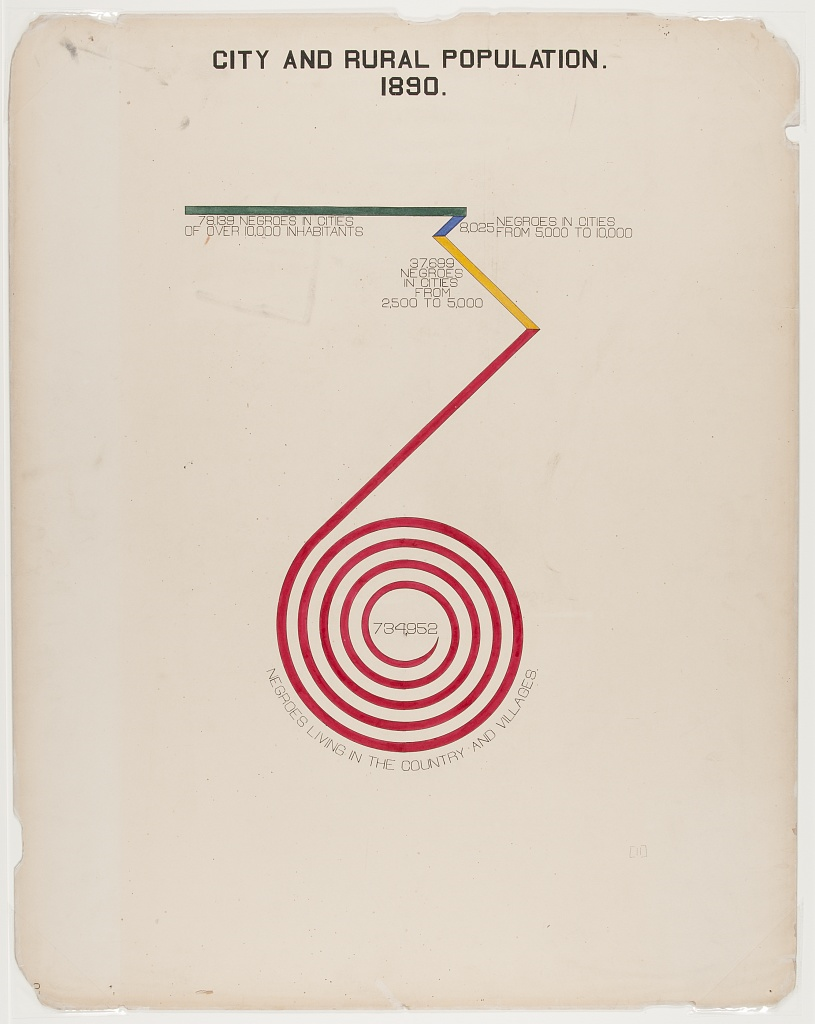
\includegraphics[width=1\textwidth]{figures/intro/du_bois_spinny.png}
        \caption{}
        \label{fig:intro_dpa}
    \end{subfigure}
    \begin{subfigure}{.24\textwidth}
        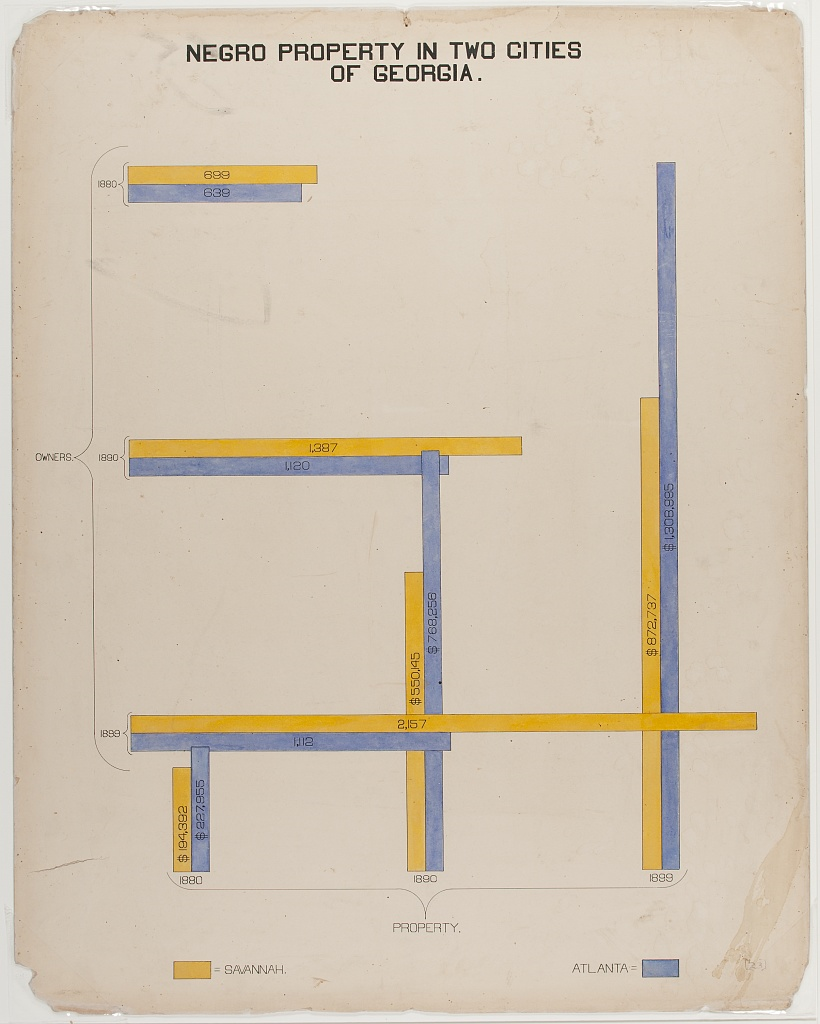
\includegraphics[width=1\textwidth]{figures/intro/du_bois_bar.png}
        \caption{}
        \label{fig:intro_dpb}
    \end{subfigure}
    \begin{subfigure}{.24\textwidth}
        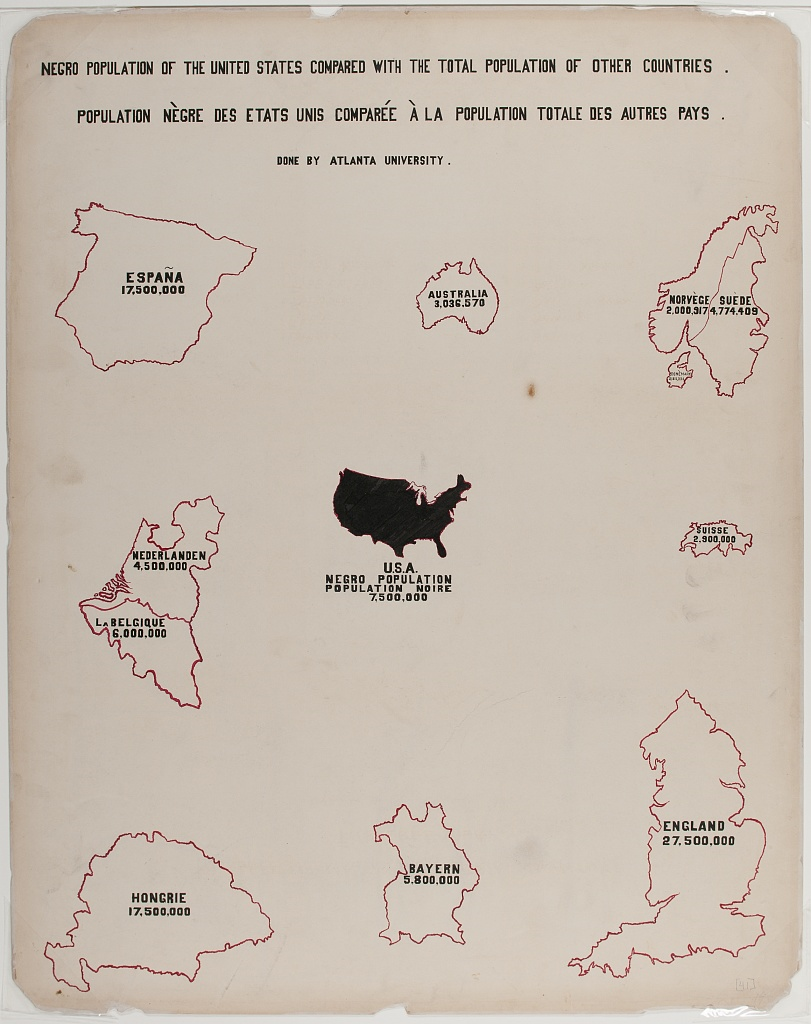
\includegraphics[width=1\textwidth]{figures/intro/du_bois_country.png}
        \caption{}
        \label{fig:intro_dbc}
    \end{subfigure}
    \begin{subfigure}{.24\textwidth}
        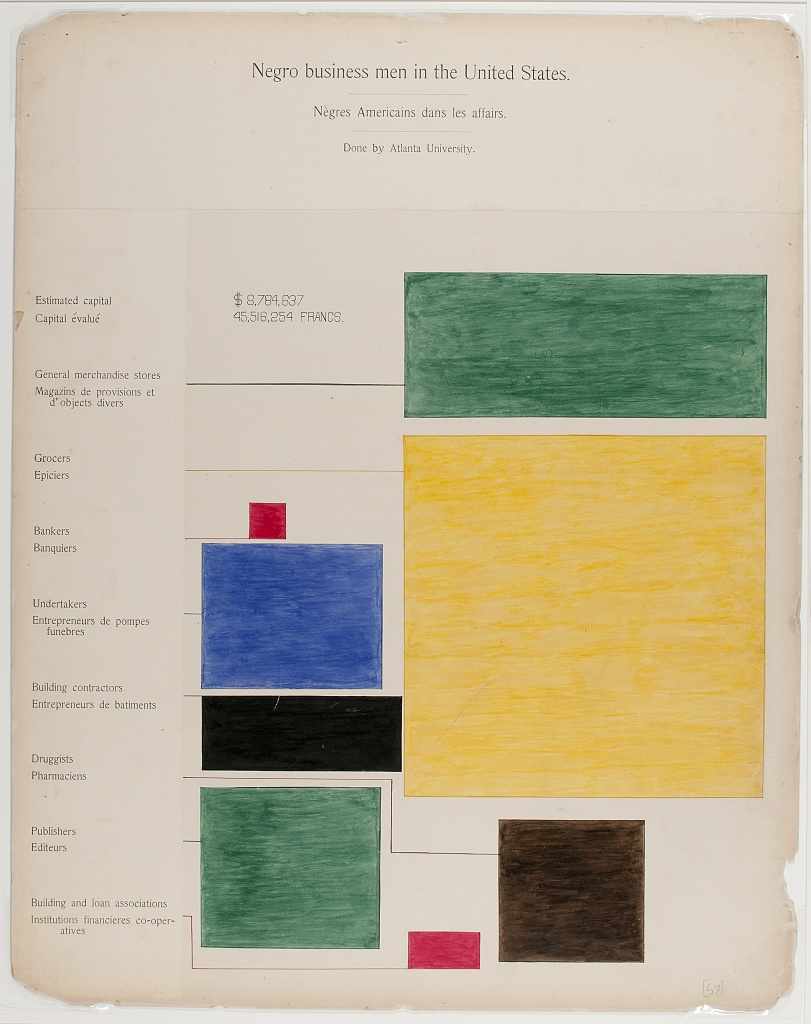
\includegraphics[width=1\textwidth]{figures/intro/du_bois_heat.png}
        \caption{}
        \label{fig:intro_dbd}
    \end{subfigure}
    \caption{Du Bois' data portraits\cite{duboiscenterattheuniversityofmassachusettsBoisDataPortraits2018} of post reconstruction Black American life exemplify that the fundemental characteristics of data visualization is that the visual elements vary in proportion to the source data. In figure~\ref{fig:intro_dpa}, the length of each segment maps to population; in figure~\ref{fig:intro_dpb}, the bar charts are intersected to show the number of property owners and how much they own in a given year; in figure~\ref{fig:intro_dpc} the countries are scaled to population size; and figure~\ref{fig:intro_dpd} is a treemap where the area of the rectangle is representative of the number of businesses in each field. The images here are from the Prints and Photographs collection of the Library of Congress \cite{duboisGeorgiaNegroCity1900,duboisGeorgiaNegroNegro1900, duboisSeriesStatisticalCharts, duboisSeriesStatisticalChartsa}}
    \label{fig:intro_dubois}
\end{figure}

This work aims to develop a model of visualization such that a tool built using this model could support visualizations as varied as those of Du Bois in figure~\ref{fig:intro_dubois}; to do so, we first discuss the criteria by which a visualization is evaluated. As described by Mackinlay, a visualization tool produces a graphical design and an image rendered based on that design. He defines the graphical design as the set encoding relations from data to visual representation, and the design evaluated on an idealized space is what throughout this paper we will refer to as graphics \cite{mackinlayAutomatingDesignGraphical1986}. Mackinlay  proposes that a visualization tool can be evaluated by its expressiveness and effectiveness; A visualization tool's expressiveness is a measure of how much of the structure of the data the tool encodes, while effectiveness describes how much design choices are made in deference to perceptual saliency \cite{clevelandResearchStatisticalGraphics1987,clevelandGraphicalPerceptionTheory1984,chambersGraphicalMethodsData1983a}. Mackinlay's definition of expressiveness is formalized at the component level, for example that ordinal values must map to ordinal positions. He uses a scatter chart for discrete data and states that a line chart must have continuous data, but does not describe how to prove this. 
While Mackinlay is strictly focusing on the graphical components of a visualization, Byrne et al. propose that visualizations also have figurative representations that have meaning due to their similarity in shape to external concepts \cite{byrneAcquiredCodesMeaning2016}. In figure~\ref{fig:intro_dbc}, Du Bois combines a graphical representation where glyph size varies by population with a figurative representation of those glyphs as the countries the data is from, which means that the semantic nominal and numerical properties of the data are preserved in the graph. Tufte specifies that visual representations must be in proportion to the quantitative data being represented for a chart to be faithful and that there should be no extra information in the graphic or figurative elements of the graph, but otherwise his notion of graphic integrity is heavily context dependent\cite{tufteVisualDisplayQuantitative2001}. As is Norman's Naturalness Principal, which states that visualizations are more understandable  when the properties of the representation match the properties of the information being represented\cite{norman_things_smart}. Bertin takes it as a given that data properties match visual properties, so much so that Munzner argues it is inherently built into his classification system \cite{munznerVisualizationAnalysisDesign2014}. In this work, we propose that this property matching can be formally defined as equivariant maps from data to graphic representation. 
 

\subsubsection{Retinal (Visual) Variables}
\label{sec:intro_visual_variables}
\begin{figure}[h!]
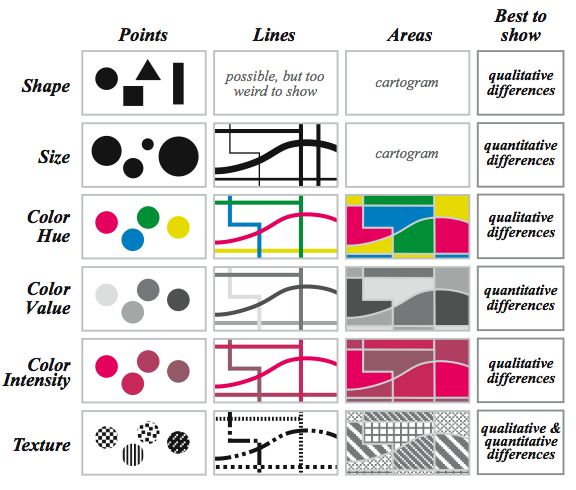
\includegraphics[width=1\textwidth]{figures/intro/retinal_variables.png}
\caption{Retinal variables are a codification of how position, size, shape, color and texture are used to illustrate variations in the \textit{components} of a visualization. This tabular form of Bertin's retinal variables is from Understanding Graphics \cite{malamedInformationDisplayTips2010} who reproduced it from \textit{Making Maps: A Visual Guide to Map Design for GIS} 
\cite{krygierMakingMapsVisual2005}}
\label{fig:retinal_variables}
\end{figure}
Figure~\ref{fig:retinal_variables} illustrates common guidelines for encoding \textit{components} of the data as components of the graphics. Bertin names these graphic components retinal variables; they are also called visual variables \cite{bertin_semiology_2011,krygier_making_2005,chambers_graphical_1983,wilkinson_grammar_2005,munzner_visualization_2014} or visual characteristics\cite{carpendaleVisualRepresentationSemiology}. The columns of figure~\ref{fig:retinal_variables} correspond to the type of observation: discrete points, continuous events (e.g. a timeseries), two dimensional continuous events (e.g. a vector map). The rows of figure~\ref{fig:retinal_variables} describe ways to visualize variations in the \textit{components}; generally, quantitative components are represented by retinal variables that change quantitatively and categorical components are represented by retinal variables that vary qualitatively. In figure~\ref{fig:iris_scatter}, the hue of the marker is used to encode differentiation in species and the position of the marker is used to show variation in petal length and sepal length. The retinal variables suggest that any single visualization is limited to encoding at most about 8 or 9 components. Retinal variables provide guidelines for encoding \textit{components}, but the choice of graph is based on the type and structure of the data. 

\section{Not all data are tables}


Tory and Moller 



"The boundary between scientific visualization and infovis has been explored by Tory and Moller [37] who note ways that discrete and continuous data and the attribute types form a design space that contains both infovis and scientific visualization." \cite{pousmanCasualInformation2007}


set up: dubois
\subsubsection{Data Type and Structure}
%% mention tidy/spivak first, set up that we use variable, record, key/index notation
%% define continuity in the math, connectivity in the data
%% topological spaces are frame in terms of continuity
% the implementation of $K$ embeds the connectivity
\label{sec:intro_data_structure}
\begin{figure}[h!]
 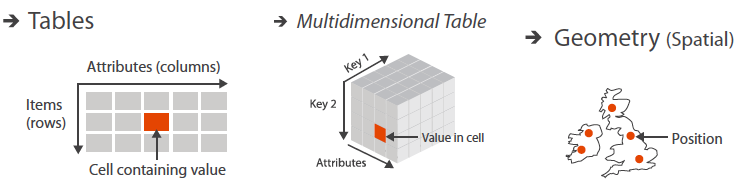
\includegraphics[width=\textwidth]{figures/intro/munzner_datatypes}
\caption{Keys are unique lookup values used to find individual observations in the dataset. Keys are positional references, and can be coordinates on a map or unique values such as a primary key in a database or a (time, latitude, longitude) index in a data cube. Image modified from a diagram from Munzner's \textit{Visualization Analysis and Design} \cite{munznerVisualizationAnalysisDesign2014}}
\label{fig:munzner_datatypes}
\end{figure}

As shown in figure~\ref{fig:flowchart}, there are multiple ways to translate data into pictures. A map is always an option, except when the observations do not have associated coordinates in a physical plane. Tamara Munzner provides a way to distinguish between these datasets using $\{key, value\}$ designations \cite{munznerVisualizationAnalysisDesign2014}. Munzner defines \textit{values} as measurements of interest in the dataset, analogous to dependent variables in statistics. She defines \textit{keys} as indexes that can be used to look up values, analogous to independent variables in statistics and dimensions in computer science. Figure~\ref{fig:munzner_datatypes} illustrates how these keys are used to look up variables in a dataset: 
\begin{itemize}
	\item map: keys are the coordinates of the points
	\item table: row index, database primary key
	\item data cube: row, column, etc. (.e.g. $i,j,k$) index
\end{itemize}

Expanding on Munzner's key and value semantics, in many datasets the keys are discrete variables like time or geophysical locations sampled from a continuous curve, surface, or field. While these observations are discrete samples from the continuous space, often the continuous (functional) characteristic\cite{ramsayFunctionalDataAnalysis2006a,mullerFunctionalVarianceProcesses2006a} of the observational space is also of interest. Besides quantitative discrete, quantitative continuous, or categorical measurement type considerations, the choice of visualization is also influenced by the measurement being on an interval, ratio, nominal, or categorical scale. 

Throughout this form we will be using the following conventions to discuss data:

\begin{description}
    \item[component]
    \item[index]  
    \item[record]
    \item[value]  
\end{description}

\subsection{how does this tackle the problem? what does it leave on the table?}
Most visualization tools are designed around some notion of the structure of the data being visualized. For example Grammer of Graphics asusmes ythat 

 
Tables, images (Lev), graphs (network X)

\begin{itemize}

    \item GoG's mathematics of visualizations
    This book focuses instead on rules for constructing graphs mathematically
and then representing them as graphics aesthetically.
The title of this book also recalls Bertin’s Semiology of Graphics (1967),
the first and most influential structural theory of statistical graphics. Bertin’s
work has pervaded our thinking. Semiology deals with signs. Although Bertin
put his signs on paper, his work applies as well to virtual space.
    \item vtk's qausi topological
    \item butler's topological formulation
\end{itemize}

\subsection{How do other visualization libraries tackle this?}
begin{figure}[h!]
%%remake properly at some point
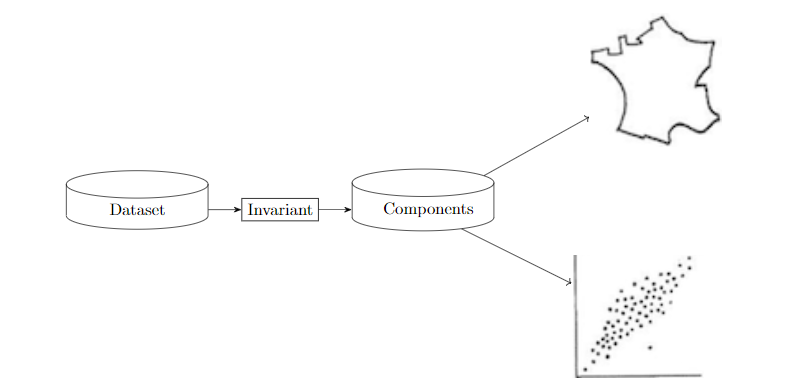
\includegraphics[width=\textwidth]{figures/intro/flowchart.png} 
\caption{To go from a dataset to a visualization, the data is subset based on a set of constraints (the invariant). The resulting subset becomes the components that are visualized, but the choice of visualization is dependent on the type and structure of the component variables.}
\label{fig:flowchart}
\end{figure}

Given a dataset, we need to decide what subset of the data to visualize. Bertin describes the set of constraints used to subset the data as the \textit{invariant}. Formally, the \textit{invariant} is the set of shared characteristics of the data being visualized. When these constraints are applied to the dataset, the resulting subset is what will become the \textit{components} of the visualization \cite{bertinSemiologyGraphicsDiagrams2011a}. 
%%rework this statement for french labor data
%%In figure~\ref{fig:iris_scatter}, the \textit{invariant} common to all the data being visualized is "sepal length", "petal length", and "species" and the \textit{components} are the measurements of these variables. 
As shown in figure~\ref{fig:flowchart}, the final step in creating a visualization is choosing how to encode the
components using retinal (visual) variables.
matplotlib arch paper, excel/matlab arch, 
vtk \& ggplot (compare/contrast, we're blending these things) 



\subsection{contribution}
The contribition of this work is a model we call the topological artist model (TAM) in which data and graphics can be viewed as sections of fiber bundles. This model allows for (1) decomposing the translation of data fields (variables) into visual channels via an equivariant map on the fibers and (2) a topology-preserving map of the base spaces that translates the dataset connectivity into graphical elements. Furthermore, this model supports an algebraic sum operation such that more complex visualizations can be built from simple ones. To demonstrate the practical value of the model, we built a prototype where we represent the topological base spaces using triangulation, make use of programming types for the fiber, and build on Matplotlib's existing infrastructure for the rendering. 
\end{document}